\documentclass[12pt, letterpaper]{article}
\usepackage{bbold}
\usepackage{dsfont}
\usepackage{indentfirst}
\usepackage{amsmath, amssymb}
\usepackage[T1]{fontenc}
\usepackage[utf8]{inputenc}
\usepackage{physics}
\usepackage{tensor}
\usepackage{braket}
\usepackage{graphics}
\usepackage{grffile}
\usepackage[export]{adjustbox}
\usepackage{svg}
\usepackage{caption}
\usepackage{subcaption}
\usepackage{authblk}
%\usepackage[dvipsnames]{xcolor}
\usepackage{setspace}
\usepackage{longtable}
\usepackage{listings}
\usepackage{xcolor}
\usepackage[framemethod=tikz]{mdframed}
%\usepackage[dvipsnames]{xcolor}
\newcommand*{\1}{\hspace{1pt}}

            \definecolor{codegreen}{rgb}{0,0.6,0}
            \definecolor{codegray}{rgb}{0.5,0.5,0.5}
            \definecolor{codepurple}{rgb}{0.58,0,0.82}
            \definecolor{backcolour}{rgb}{0.95,0.95,0.92}

            \lstdefinestyle{mystyle}{
                backgroundcolor=\color{backcolour},   
                commentstyle=\color{codegreen},
                keywordstyle=\color{magenta},
                numberstyle=\tiny\color{codegray},
                stringstyle=\color{codepurple},
                basicstyle=\ttfamily\footnotesize,
                breakatwhitespace=false,         
                breaklines=true,                 
                captionpos=b,                    
                keepspaces=true,                 
                numbers=left,                    
                numbersep=5pt,                  
                showspaces=false,                
                showstringspaces=false,
                showtabs=false,                  
                tabsize=2
            }

            \lstset{style=mystyle}

\title{\Huge{Out-of-Time-Order-Correlator of $H=xp$}}
\author{Noor E Mustafa Ferdous}

\begin{document}
    
    \maketitle
    %\doublespacing
    \newpage
    \section*{Out-of-Time-Order-Correlator of $H=xp$}
    \bibliographystyle{unsrt}
    \begin{abstract}
        Bery-Keating Hamiltonian $H_{0}=\frac{1}{2}(xp+px)$ resembles the Hilber-P$\acute{o}$lya 
        cojectue of Riemnan Hypothesis, shows quantum chaotic behaviour. In this paper we first 
        quantize xp and adding boundary condition evalute spectrum with proper eigenfucntion.
        Then we quantutize 1/xp and achieve same spectrum with minor phase addition. We observes
        OTOC of the hamiltonian, which gauge the quantum chaotic behaviour of it.
    \end{abstract}

    \newpage

    \tableofcontents

    \newpage
    %\begin{mdframed}[hidealllines=true,backgroundcolor=blue!20]
    \section{Introduction}
    The Riemann hypothesis states that non-trivial zeros of the classical zeta function have real part equal to 1/2. The classical zeta function converges at
    Re $s > 1$ . By the fundamental theorem of arithmatic, which is also equivalent to the Euler product over primes where p are all the prime numbers. So zeta 
    can describe all the prime numbers.Also the zeros of Riemann zeta function are two different types. Trivial zeros of zeta / Riemann zeta function occurs at all negetive integers (for $s = -2, -4, -6, .......$). 
    For complex s (=$\sigma + it $) (with real part between zero and one) , zeta fucntion becomes nontrivial ones. And the Riemann hypothesis is for $s=\frac{1}{2}-iE$
    zeta funtion becomes zero. If the Riemann hypothesis is true the statistical distribution of the primes will be constrained 
    in the most favourable way. Hilbert-P$\acute{o}$lya conjecture suggests that the imaginary parts of the nontrivial zeros are the eigenvalues 
    of a self-adjoint hamiltonian operator $\hat{H}$. It is also one of the aprroach to proving the Riemann hypothesis. Berry-Keating conjectured that the hamiltonian operator
    of the Hilbert-P$\acute{o}$lya  conjecture should take the form\cite{s1}$\hat{H} _{BK} = \frac{1}{2}(\hat{x}\hat{p} + \hat{p}\hat{x})$.
    The classical versus quantum version of primes and the zeros is also at the heart of so-called quantum chaos approach to the RH.

    Here x and p are position and momentum operators. This 1d classical Hamiltonian ($H = xp$) related to the Riemann zeros.\cite{s1}
    In 1999, Berry and Keating\cite{s1,s15} on the one hand and Connes\cite{s3} on the other claimed that the classical Hamiltonian H = xp, 
    where x and p are the location and momenta of a 1D particle, is strongly connected to the Riemann zeros. This startling 
    hypothesis was based on a semiclassical analysis of H = xp, which led these authors to very different conclusions about 
    the probable spectral interpretation of the Riemann zeros. The source of the dispute is the use of distinct 
    regularizations of H = xp. Berry and Keating used a Planck cell regularization, in which the smooth component of the
    Riemann zeros is represented semiclassically as discrete energy levels. Connes, on the other hand, chose an upper 
    cutoff for the position and momenta, resulting in a semiclassical continuous spectrum devoid of smooth zeros.
    All of these semiclassical solutions are heuristic, and there is no consistent quantum version as of yet.



    The out-of-time-order correlator (OTOC) is typically defined by \cite{s11}

    \begin{equation}
        C_{T} \equiv  - \left\langle\left[W(t),V(0)\right]^{2}\right\rangle
    \end{equation}

    where $<\cdot \cdot \cdot >$ represents the thermal average. W(t) and V(t) are operators as time in t in the Heisenberg representation. The OTOC, first introduced
    in a calculation of a vertex correction of a current for a superconductor\cite{s12}, was recently turned out to be considered as a measure of the magnitude of 
    quantum chaos. A naive argument for the relation between the OTOC and chaos is as follows\cite{s13}. Consider poistion and momentum operators, x(t) and p(t), in a
    quantum system. We can define an OTOC as $C_{T} = - \left\langle\left[x(t),p(0)\right]^{2}\right\rangle$. Taking a naive semiclassical limit, we would be able to 
    replace the commutator $\left[x(t),p(0)\right]$ by the Poissoin bracket $i\hbar\{x(t),p(0)\}_{PB} = i\hbar\frac{\delta x(t)}{\delta x(0)}$. For a classically 
    chaotic system with a Lyapunov exponent $\lambda$, we have $\frac{\delta x(t)}{\delta x(0)}\thicksim  e^{\lambda t}$ because of sensiitivity to initial condition.
    Thus, the OTOC should grow as $\thicksim \hbar^{2}e^{2\lambda t}$ and we can read off the quatnum Lyapunov exponent $\lambda$ form it. The quantization of a 
    classically chaotic system may provide a positive quanutm Lyapunov exponent of the OTOC. Historically, the nearest neighbour distribution (NND) for the energy
    level spectrum has been used to quantify quantum chaos \cite{s14}. For integrable and non-integrable systems, it is considered that NNDs are given by Poission
    and Wigner distributions. The OTOC is expected to be another measure of qauntum chaos. A possible distinction from the classical chaotic system is that the 
    OTOC does not grow eternally but saturates at the Ehrenfest time $t_{E}$. The Ehrenfest time is defined by the time scale beyond which the wave function spreads
    over the whole system. It is roughly characterized as a boundary between a particle-like behavior and a wave-like behavior of the wave function.

    In the definition of OTOC, we consider the thermal average of $- \left\langle\left[W(t),V(0)\right]^{2}\right\rangle$. When we take thermal average, we need to 
    consider the four point operator $\left\langle\left[W(t),V(0)\right]^{2}\right\rangle$ instead of two point operator $\left\langle\left[W(t),V(0)\right]\right\rangle$.
    The reason is as follows. Assuming that we can replace the commutator by Poission bracket by semiclassical limit, $\left\langle\left[W(t),V(0)\right]\right\rangle$
    would also show the exponential growth $\thicksim  e^{\lambda t}$. However, its coefficient can be both positive and negetive. By taking the thermal average, their
    contributions would be canceled. From the quantum theory point of view, $\left\langle\left[W(t),V(0)\right]\right\rangle$ measures the correlation between W(t)
    and V(0). Therefore, the two point function decays as $t \rightarrow \infty$ and cannot show the chaotic behavior.

    %\end{mdframed}
    Now we look into the Berry-Keating and Connes semiclassical approaches to $H=xp$

    \section{Semiclassical approach}

    The classical Berry-Keating-Connes (BKC) Hamiltonian is\cite{s1,s2}

    \begin{equation}
        H ^{cl} _{0} = xp
    \end{equation}

    which has hyperbolic trajectories 
    
    \begin{equation}
        x(t) = x_{0}e^{t}  \ \ \ \  p(t) = p_{0}e^{-t}
    \end{equation}

    So the dynamics is unbounded. There is a continuous spectrum as the quantum level. Berry-Keating and Connes introduced two different types of reularizations and counted
    the semiclassical states. Berry-Keating introduced Plank cell in a phase space: $|x| > l_{x}$ and $|p| > l_{p}$, with $l_{x}l_{p} = 2 \pi \hbar$. Connes 
    choosed $|x| < \Lambda $ and $|p| < \Lambda$, where $\Lambda$ is a cutoff. German Sierra introduced us a third regularization, $l_{x} < x < \Lambda$ combines
    the Berry-Keating and Connes regularization position, not taking assumptions for the momenta p. \

    Semiclassical states number $\mathcal {N}(E)$ with an enery between 0 to E is given by
    \begin{equation}
        \begin{split}
            \mathcal {N}(E) &= \frac{A}{2 \pi \hbar} \\
            &= \frac{A}{h}
        \end{split}
    \end{equation}

    Where A is the area of the allowed phase space region below the curve $E = xp$.

    %\begin{mdframed}[hidealllines=true,backgroundcolor=blue!20]
    \begin{adjustbox}{center,caption={Berry-Keating Regularization},label={microcanocnial OTOC},nofloat=figure,}
        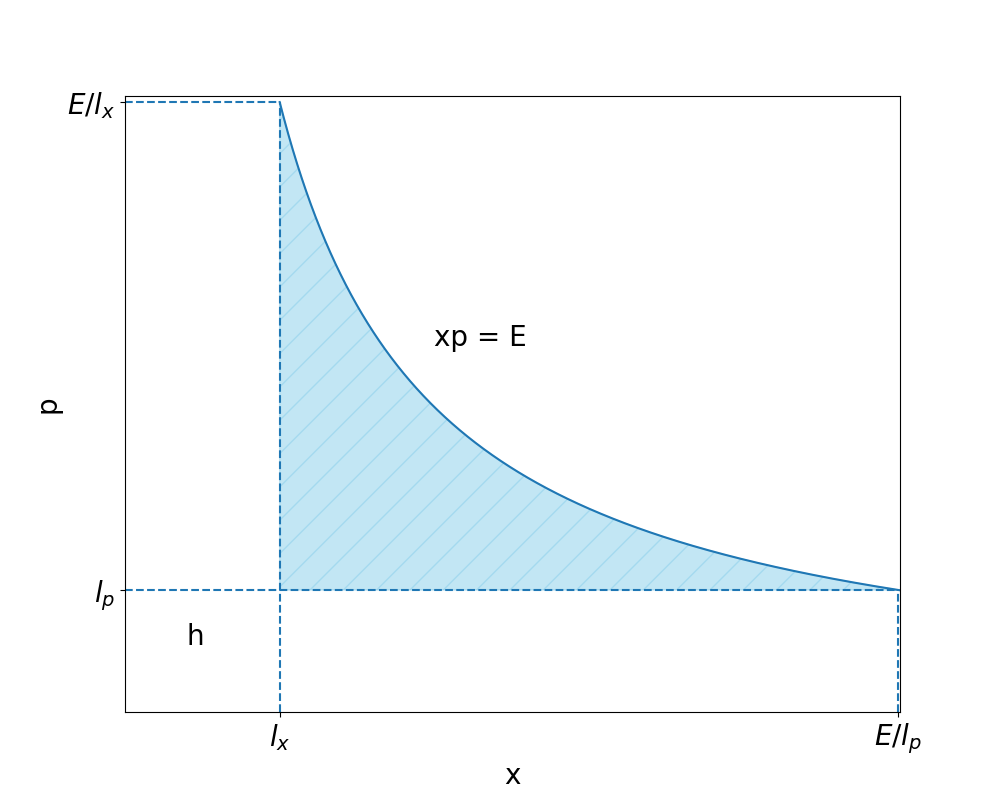
\includegraphics[width=0.6\textwidth]{pic4}
    \end{adjustbox}

    \begin{adjustbox}{center,caption={Connes Regularization},label={microcanocnial OTOC},nofloat=figure,}
        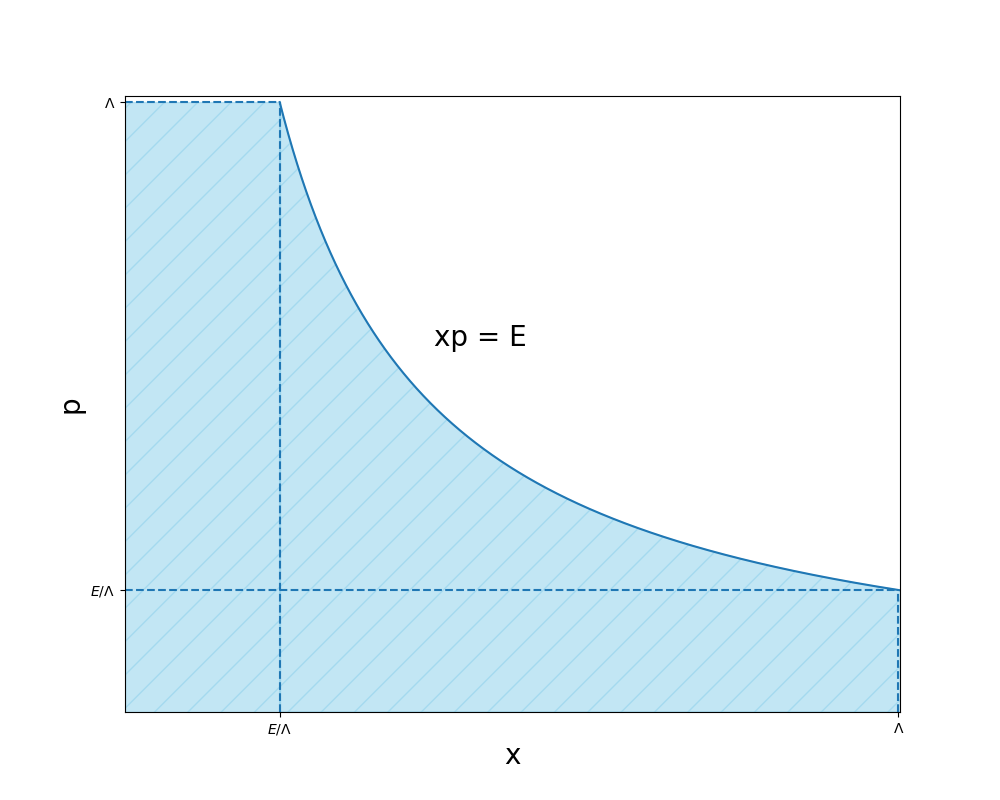
\includegraphics[width=0.6\textwidth]{pic3}
    \end{adjustbox}
    %\end{mdframed}

    So the the number of semiclassical states will be for Berry-Keating regularization 
    \begin{equation}
        \begin{split}
            \mathcal {N}_{BK}(E) &= \frac{1}{h}\int_{l_{x}}^{\frac{E}{l_{p}}}  \,dx \int_{l_{p}}^{\frac{E}{x}}  \,dp + ....... \\
            &= \frac{1}{h}\left[\int_{l_{x}}^{\frac{E}{l_{p}}}  \,dx \left[\frac{E}{x} - l_{p}\right] \right]  \\
            &= \frac{1}{h}\left[E\left[\ln x\right] ^{\frac{E}{l_{p}}} _{l_{x}} - l_{p}\left[\frac{E}{l_{p}} - l_{x}\right] \right]  \\
            &= \frac{1}{h}\left[E\ln \frac{E}{l_{x}l_{p}}  - E - l_{x}l_{p} \right]  \\
            &= \frac{1}{h}\left[E\ln \frac{E}{l_{x}l_{p}}  - E - h \right]  \\
            &= \frac{E}{h}\left[\ln \frac{E}{l_{x}l_{p}}  - 1 \right]  + 1 \\
            &= \frac{E}{2 \pi \hbar}\left[\ln \frac{E}{2 \pi \hbar}  - 1 \right]  + 1 \\
        \end{split}
    \end{equation}

    adding Maslov phase $(-\frac{1}{8})$ and $\hbar = 1$, it becomes 
    \begin{equation}
        \mathcal {N}_{BK}(E) = \frac{E}{2 \pi}\left[\ln \frac{E}{2\pi}  - 1 \right]  + \frac{7}{8} + .......,  \ \ \ \ \ \ E>>1\\
    \end{equation}

    The exact formula for the Riemann zeros, $\mathcal{N}_{R} (E)$ contains a fluctuation term which depends on the zeta funcion.\cite{s3}  
    \begin{equation}
        \begin{split}
            \mathcal{N}_{R} (E) &= \left\langle \mathcal{N}\right\rangle + \mathcal{N}_{fl} (E) \\
            \left\langle\mathcal{N} (E)\right\rangle &= \frac{1}{\pi} Im \ ln \left[\Gamma\frac{1}{2}\left(\frac{1}{2}-iE\right) \right] - \frac{E}{2 \pi} ln \pi + 1  \\
            \mathcal {N} _{fl} (E) &= \frac{1}{\pi} Im \ ln \left[\zeta\left(\frac{1}{2} - iE \right)\right]
        \end{split}
    \end{equation}

    Bery-Keatin took this result and analogies between formulae in Nunber Theory and Quantum Chaos, they pointed the quantization of classical chaotic Hamiltonian give
    rise to the zeros as point like spectra.\cite{s1,s4} Whereas Connes found the number of semicassical states diverges in the limit where the cutoff $\Lambda$ goes to
    infinity, and that therre us a finite size correction given by mins the average position of the Riemann zeros.

    \begin{equation}
        \begin{split}
            \mathcal {N}_{c} (E) &= \frac{1}{h}\left[ 2E - \left(\frac{E}{\Lambda} \right)^{2} + \int_{\frac{E}{\Lambda}}^{\Lambda}  \,dx\int^{\frac{E}{x}}_{\frac{E}{\Lambda}}  \,dp   \right] \\ 
             & = \frac{1}{h}\left[ 2E - \left(\frac{E}{\Lambda} \right)^{2} + \int_{\frac{E}{\Lambda}}^{\Lambda}  \,dx\left[\frac{E}{x} - \frac{E}{\Lambda}\right]   \right] \\ 
             & = \frac{1}{h}\left[ 2E - \left(\frac{E}{\Lambda} \right)^{2} + E\left[ln \ x\right] _{\frac{E}{\Lambda}}^{\Lambda} - \frac{E}{\Lambda}\left[\Lambda - \frac{E}{\Lambda}\right]   \right] \\ 
             & = \frac{1}{h}\left[ 2E - \left(\frac{E}{\Lambda} \right)^{2} + E\left[ln \ \frac{\Lambda ^{2}}{E}\right] - E + \left(\frac{E}{\Lambda}\right)^{2}\right]  \\ 
             & = \frac{1}{h}\left[ E  + E\left[ln \ \frac{\Lambda ^{2}}{E}\right] \right]  \\ 
             & = \frac{1}{h}\left[ E  + E\left[ln \ \frac{\Lambda ^{2}}{E}\frac{2\pi}{2\pi}\right] \right]  \\ 
             & = \frac{E}{h} ln \ \frac{\Lambda ^{2}}{2\pi} - \frac{E}{h} \left[ln \ \frac{E}{2\pi} - 1\right]  \\
             & = \frac{E}{2\pi} ln \ \frac{\Lambda ^{2}}{2\pi} - \frac{E}{2\pi} \left[ln \ \frac{E}{2\pi} - 1\right] \ \ \ \ \ \ \ \ \ \ \ \ \ \ \ \ \   [taking \ \ \hbar=1] \\
        \end{split} 
    \end{equation}

    This result les to the missing spectral interpretation of the Riemann zeros, according to which there is a continuum of eginstates (represented by the term $\frac{E}{\pi}
     ln \ \Lambda$ in $\mathcal {N} (E)$) where states asscoiated with Riemann zeros are missing.

    Finally, in the S-regularization the number of semiclasical states diverges as $\frac{E}{2\pi} \ ln \ \frac{\Lambda}{l_{x}}$ suggesting a continuum spectrum, ike in 
    Connes's approach. But there is no finite size correction to that formula, and cosequently the possible connection to the Riemann zeros is lost. \\ 
    \\ 
    \\


    \begin{longtable}[c]{c c c }
        \caption{\\Three different regularizations of $H=xp$ and the corresponding number of semiclassical states in units $\hbar=1$\cite{s7} }\\
        \hline
         Type & Regularization & $\mathcal{N}(E)$\\
         \hline 
         BK & $|x| > l_{x}, |p| > l_{p}$ & $\frac{E}{2\pi}\left(ln \ \frac{E}{2\pi}-1\right)+1$  \\  
         C & $|x| < \Lambda, |p| < \Lambda$ & $\frac{E}{2\pi}ln \ \frac{\Lambda^{2}}{2\pi} - \frac{E}{2\pi}\left(\ln \ \frac{E}{2\pi}-1\right)$   \\ 
         S & $l_{x} < x < \Lambda$ & $\frac{E}{2\pi}ln \ \frac{\Lambda}{l_{x}}$   \\ 
        \hline
    \end{longtable}
    \section{Quantization of xp and $\frac{1}{xp}$}
    
    
    \subsection{The Hamitoninan $H_{0} = xp$}

        Here we construst a self adjoint operator $H_{0}$ which acts on a Hilbert space $L^{2}(a,b)$ of square integrable function in the interval $(a,b)$. Taking $x\geqslant 0$
        , there are four possible intervals: $a=0,l_{x}$ and $b=\Lambda, \infty $ where $l_{x}$ and $\Lambda$ were introduced (we shall take $l_{x}$ and $\Lambda = N > 1$).
        Berry-Keating defined the quantnum Hamiltonian $H_{0}$ as the normal ordered expresion 

        \begin{equation}
            H_{0} = \frac{1}{2}(xp + px)
        \end{equation}

        where $p = -i\hbar \frac{d}{dx}$. If $x\geqslant 0$, Eq. (11) is equivalent to

        \begin{equation}
            \begin{split}
                H_{0} &= \sqrt{x} p \sqrt{x} = -i\hbar \sqrt{x} \frac{d}{dx} \sqrt{x}\\ 
                &= -i\hbar\left(x\frac{d}{dx}+\frac{d}{dx}x\right)
            \end{split}
        \end{equation}

        We know that the canonical commutation relation is 
        
        \begin{equation}
            \left[\hat{x},\hat{p}\right] = i\hbar
        \end{equation}
        
        or, (dropping hat cause we're dealing with quantum system and operators)
        \begin{equation}
            \begin{split}
                \left[x,p\right] &= i\hbar \\ 
                \implies \left[x,-i\hbar\frac{d}{dx}\right] &= i\hbar \\
                \implies -i\hbar\left[x,\frac{d}{dx}\right] &= i\hbar \\
                \implies \left[x,\frac{d}{dx}\right] &= -1 \\
                \implies x\frac{d}{dx} - \frac{d}{dx}x &= -1 \\
                \implies  \frac{d}{dx}x &= x\frac{d}{dx} + 1 \\
            \end{split}
        \end{equation}

        Taking this value to R.H.S of Eq(12)

        \begin{equation}
            \begin{split}
                -i\hbar\left(x\frac{d}{dx} + \frac{d}{dx}\right)f &= -i\hbar\left[2x\frac{d}{dx}+1\right] \\ 
                & = -i\hbar2x\left[\frac{d}{dx}+\frac{1}{x}\frac{1}{2}\right]f \\ 
                & =  -i\hbar\frac{1}{\sqrt{x}}\frac{d}{dx}\left(\sqrt{x}f\right) \\ 
                & =  -i\hbar\frac{1}{\sqrt{x}}\frac{d}{dx}\left(\sqrt{x}f\right) \\ 
                & =  \frac{1}{\sqrt{x}}\left(-i\hbar\frac{d}{dx}\right)\sqrt{x}f \\ 
            \end{split}
        \end{equation}

        so 
        \begin{equation}
            H_{0} = \frac{1}{2}\left(xp + px\right) = -i\hbar\sqrt{x}\frac{d}{dx}\sqrt{x}
        \end{equation}
        

        This is a symmetric operator acting on a certain domain of the Hilert space $L^{2}(a,b)$, By definition, if an operator is symmetric (or Hermitian)\cite{s5}

        \begin{equation}
            \left\langle\psi | H_{0}\phi \right\rangle = \left\langle\psi H_{0} |\phi \right\rangle
        \end{equation}
         or with limit,
        \begin{equation}
            \left\langle\psi | H_{0}\phi \right\rangle - \left\langle\psi H_{0} |\phi \right\rangle = i \hbar \left[a\psi ^{*}(a)\phi(a) - b\phi ^{*}(b)\psi(b)\right] = 0
        \end{equation}
        
        which is satisfied if both $\psi (x)$ and $\phi (x)$ vanish at the points a, b. von Neumann Theorem of deficiancy indices states that, an operator in symmetric if its deficiency
        indices $n_{\pm }$ are equal.\cite{s6}. Deficiency indices (or the defect numbers) of a closable symmetric operator T are cardinal number S

        \begin{equation}
            \begin{split}
                n_{+} &:= d_{\lambda}  = dim \ \mathcal{R} (T-\overline{\lambda}\mathds{1})^{\perp }  \ \ \ \    Im \ \lambda > 0 \\
                n_{-} &:= d_{\lambda}  = dim \ \mathcal{R} (T-\overline{\lambda}\mathds{1})^{\perp }  \ \ \ \    Im \ \lambda < 0 
            \end{split}
        \end{equation}

        If T is densly defined and symmetric, then T is closable, and by formula $\mathcal{N}(T^{*}) = \mathcal{R}(T)^{\perp}$
        \begin{equation}
            \begin{split}
                n_{+} &:= dim \ \mathcal{N} (T^{*}-i\mathds{1})  = dim \ \mathcal{N} (T^{*}-\lambda \mathds{1})  \ \ \ \    Im \ \lambda > 0 \\
                n_{-} &:= dim \ \mathcal{N} (T^{*}+i\mathds{1})  = dim \ \mathcal{N} (T^{*}+\lambda \mathds{1})  \ \ \ \    Im \ \lambda < 0 
            \end{split}
        \end{equation}

        By definition $n_{\pm} (T) = dim \ \mathcal{N}(T^{*} \mp iT )$ 

        Again if T is a symmetric operator, then
        \begin{equation}
            \begin{split}
                K_{+} &= ker \ (i\mathds{1}-T^{*}) = Ran \ (i\mathds{1} - T) ^{\perp} \\
                K_{-} &= ker \ (i \mathds{1} +T^{*}) = Ran \ (-i\mathds{1} + T) ^{\perp} \\ 
            \end{split}
        \end{equation}
        
        $K_{+}$ and $K_{-}$ are called the deficiency subspaces of T, The pair of numbers $n_{+}$, $n_{-}$ given by $n_{+}(T) = dim[K_{+}]$,$n_{-}(T) = dim[K_{-}]$ arre called
        deficiency indices of T.

        von Neumann Theorem for deficiency indices states that if T an closed operator woth deficiency indices $n_{+}$ and $n_{-}$. Then \\ 
        \\
         (1) T is symmetric if and only if $n_{+} = n_{-} = 0$ ann self adjoint if $\mathcal{D}(T)=\mathcal{D}(T^{*})$ \\ 
         \\ 
         (2) T is symmetric adn self adjoint and also has many self adjoint extensions if and only if $n_{+}=n_{-}\neq 0$ and  $\mathcal{D}(T)=\mathcal{D}(T^{*})$.
         There is one-one correspondence between self adjoint extensions of T and unitary maps from $K_{+}$ onto $K_{-}$ \\ 
         \\ 
         (3) If either $n_{+}=0 \neq n_{-}$ or $n_{-}=0 \neq n_{+}$ then T is not symmetric and has no nontrivial self adjoint extension (such operators are called 
         maximal symmetric operator). \\
         \\
        So this indices counts the number of solutions of the equation, which comes from the deficiency spaces for subsystem T

        \begin{equation}
            K_{\pm} = ker \left(-H_{0}^{\dagger} - \mp i \mathds{1}\right)
        \end{equation}

        which leads to find the solution of the equation.
        \begin{equation}
            H_{0} ^{\dagger} \psi_{\pm} = \pm i \hbar \lambda \psi_{\pm}
        \end{equation}

        belonging to the domain og $H_{0}^{\dagger}(\lambda>0)$. If $n=n_{+}=n_{-}>0$, there are infinitely many self-adoint extensions of $H_{0}$ parameterized by a 
        unitary $n\times n$ matrix. Stone's theorem states that if $U(t)$ be a strongly continuous one parameter unitary group on a Hilbert space $\mathcal{H}$. 
        Then, there is a self-adjoint operator A on $\mathcal{H}$ so that $U(t) = e^{itA}$. The solution of the equation () is 

        \begin{align*}
            H_{0}^{\dagger} \psi_{\pm} &= \pm i \hbar \lambda \psi_{\pm} \\ 
            \implies H_{0} \psi_{\pm} &= \pm i \hbar \lambda \psi_{\pm} \ \ \ \ \ [becuase\ H_{0} \ is \ self-adjoint] \\
            \implies \left(-i\hbar \sqrt{x} \frac{d}{dx}\sqrt{x}\right)\psi_{\pm} &= \pm i \hbar \lambda \psi _{\pm} \\
            \implies -i\hbar \sqrt{x} \frac{d}{dx}\left(\sqrt{x}\psi_{\pm}\right) &= \pm i \hbar \lambda \psi _{\pm} \\
            \implies -\sqrt{x} \frac{d}{dx}\left(\sqrt{x}\psi_{\pm}\right) &= \pm \lambda \psi _{\pm} \\
            \implies -x\frac{d}{dx}\psi_{\pm} - \sqrt{x}\frac{1}{2\sqrt{x}} \frac{d}{dx}\psi_{\pm} &= \pm \lambda \psi _{\pm} \\
            \implies -x\frac{d}{dx}\psi_{\pm} &= \left(\pm \lambda + \frac{1}{2}\right) \psi _{\pm} \\
            \implies \frac{d}{dx}\psi_{\pm} &= -\frac{1}{x}\left(\pm \lambda + \frac{1}{2}\right) \psi _{\pm} \\
            \implies \frac{d\psi_{\pm}}{\psi_{\pm}} &= -\frac{dx}{x}\left(\pm \lambda + \frac{1}{2}\right) \\
            \implies ln \ \psi_{\pm} &= -\left(ln \ x\right)\left(\pm \lambda + \frac{1}{2}\right) + ln \ C\\
            \implies \psi_{\pm} &=  Cx^{- \frac{1}{2}\mp \lambda}\\
        \end{align*}

        whose norm in the interval (a,b) is
        \begin{equation}
            \begin{split}
            \left\langle \psi_{\pm} | \psi_{\pm} \right\rangle &= \int_{a}^{b} C^{2} x^{-1\mp \lambda} \,dx \\
            &= \mp \frac{C^{2}}{2\lambda}\left(b^{\mp 2\lambda} - a^{\mp 2\lambda}\right) \\  
            &= \pm \frac{C^{2}}{2\lambda}\left(a^{\mp 2\lambda} - b^{\mp 2\lambda}\right) 
            \end{split}
        \end{equation}
        The deficiency indices correponding to the four intervals cosidered above are collecte in Table\cite{s8}. We find the deficency indices by observing different intervals.
        For BK intervals$(1,\infty)$ only $\psi_{+}$ belongs to Hilbert space ($\psi_{-}$ blows out. or putting intervals in Eq. (20) and testing whether it belongs to
        the Hilbert space)\cite{s7}. And the rest are given below
        
        \begin{longtable}[c]{c c c c c}
            \caption{Deficiency indices of $H_{0}$. The corresponding intervals are associated to the semiclassical regularizations of section 2 (BK, C ,S).
            The last one T, describes the case with no constraints on x except positivity (i.e. x>0)} \\
            \hline
             Type & (a,b) & $(n_{+}, n_{-})$ & Self-adjoint\\
             \hline 
             BK & $(1,\infty)$ & (1,0) & -\\  
             C & (0,N) & (0,1) &  -\\ 
             S & (1,N) & (1,1) & $\surd$ \\ 
             T & $(0,\infty)$ & (0,0) & $\surd $\\ 
            \hline
        \end{longtable}


        From the von Neumann theorem we see that $H_{0}$ is essentially self-adjoint on the half line $\mathbb{R} _{+} = (0, \infty)$. This was studied by Twamley and Milbrn, who
        defined quantum Mellin transform using the eigenstates of $H_{0}$\cite{s9}
        On the other hand, in the interval (1,N) the operator $H_{0}$ admits infinitely many self-adjoint extensions parameterrized y a phase $e^{i\theta}$. This phase defines the 
        boundary condition of the functions belonging to the self-adjoint domain.\cite{s7}

        \begin{equation}
             \mathcal{D}(H_{0,\theta}) = \left\{\psi, H_{0}\psi \in  L^{2} (1, N), e^{i\theta}\psi(1) = \sqrt{N}\psi(N)\right\}
        \end{equation}

        The eigenfunction of $H_{0}$ 

        \begin{equation}
            H_{0}\psi_{E} = E \psi_{E},
        \end{equation}

        are given by \cite{s1}

        \begin{equation}
            \psi _{E} (x) = \frac{C}{x^{\frac{1}{2}-iE\hbar}} , \ \ \ \ E \in \mathbb{R} 
        \end{equation}

        where C is a normalization constant. In the half line $\mathbb{R}_{+}$ there are no further restriction on E, hence the spectrum of $H_{0}$ is continuous 
        and covers the whole real line $\mathbb{R}$. In this case the normalization constant is chosen as $C = \frac{1}{\sqrt{2\pi\hbar}}$ which gurantees the standard 
        normalization
        \begin{equation}
            \left\langle\psi_{E}|\psi_{E^{'}}\right\rangle = C^{2} \int_{0}^{\infty} \frac{dx}{x} x^{-i(E-E^{'})/\hbar} = \delta (E-E^{'}) 
        \end{equation}

        In the case where $H_{0}$ is defined in ther interval, the boundary condition (21) yeilds the quantization condition for E, namely

        \begin{equation*}
            \begin{split}
                e^{i\theta} \psi(1) & = \sqrt{N}\psi(N) \\ 
                \implies e^{i\theta} \frac{C}{1^{\frac{1}{2}-iE\hbar}}&= \sqrt{N}\frac{C}{N^{\frac{1}{2}-iE\hbar}} \\ 
                \implies e^{i\theta} & = N^{-iE\hbar} \\ 
                \implies i\theta & = (\frac{-iE}{\hbar})ln \ N \\
                \implies E & = \frac{\hbar\theta}{ln \ N} \\
                \implies E & = \frac{2\pi\hbar}{ln \ N}( \frac{\theta}{2\pi}) \\
            \end{split}
        \end{equation*}

        \begin{equation}
            \implies E_{n}  = \frac{2\pi\hbar}{ln \ N}(n+\frac{\theta}{2\pi})  \ \ \ \ n \in \mathbb{N}\\
        \end{equation}
        Hence the spectrum of $H_{0}$ is dscrete, with a level spacing decreasing for largerm values of N. The normalization constant of the wave function is now 
        $C = \frac{1}{\sqrt{ln \ N}}$ which gives,

        \begin{equation}
            \left\langle\psi_{E_{n}}|\psi_{E_{n'}}\right\rangle = C^{2} \int_{1}^{N} \frac{dx}{x} x^{-i(E_{n}-E_{n'})/\hbar} = \delta_{n,n^{'}}
        \end{equation}
        
        The spectrum (16) agrees with the semiclassical result given in Table 1 for the S-regularization(recall that $l_{x} = 1, \Lambda = N, \hbar=1$)
        For the particular case where $\theta=\pi$, one observes that the energy spectrum is symmetric around zero, i.e, if $E_{n}$ is an eigenenergy so is $-E_{n}$.
        This result is obtained in working\cite{s10} with the inverse Hamiltonian $\frac{1}{H_{0}}$. We are reviewing that construction in next section.

        \subsection{The inverse Hamiltonain $1/H_{0}$}

        First, we take the expression at Eq(16) and take the formal inverse, i.e., $H_{0} ^{-1} = x^{1/2}p^{-1}x^{-1/2}$. The operator $p_{-1}$ is the one-dimensional
        Green's function with matrix elements(definition of Green's function: Green's function is the kernel of and integral operator that represents the inverse
        of a differential operator. Let 

        \begin{equation}
                Lu = f
        \end{equation}

        Here u and f are vectors and L is a square, invertible matrix. The inverse matrix exsits if $\lambda=0$ is not an eigenvalue of L, or when det $det L \neq 0$.
        Now

        \begin{equation}
            u = L^{-1}f
        \end{equation}

        where $L^{-1}$ is the inverse operator of L. The inverse operator to be an integral operator of the form.

        \begin{equation}
            \left(L^{-1}f\right)(x) = \int_{a}^{b} g(x,\xi ) f(\xi) \,d\xi 
        \end{equation}

        with kernel G. If L exists, then the kernel fucntion $g(x,\xi)$ is called the Green's function associated with L.

        So $p^{-1}$ operator will be
        \begin{equation}
            \begin{split}
                \left\langle x\middle|p^{-1}\middle|x^{'}\right\rangle &= \left\langle x\middle| \frac{1}{-i\hbar\frac{d}{dx}}\middle| x^{'}\right\rangle \\ 
                &= -i\hbar\left\langle x\middle| \frac{1}{\frac{d}{dx}}\middle| x^{'}\right\rangle \\
                &= \frac{\hbar}{i}G(x,x^{'}) \\ 
                &= \frac{\hbar}{2i} sign(x-x^{'})
            \end{split}
        \end{equation}

        Here $sign(x-x^{'})$ is the sign function.\cite{s10}. The operator $H_{0}^{-1}$ is defined in the interval (1,N) by the continuous matrix,

        \begin{equation}
            H_{0} ^{-1} (x,x^{'}) = \frac{i}{2\hbar} \frac{sign(x-x^{'})}{\sqrt{x x^{'}}},  \ \ \ \ 1\leqslant x , x^{'} \leqslant N.
        \end{equation}

        It's spectrum is found solving the Schr$\ddot{o}$dinger equation. 

        \begin{equation}
            \begin{split}
                &H_{0}(x,x^{'}) \psi(x^{'}) = E \psi(x) \\ 
                & \implies H_{0} ^{-1}(x,x^{'}) \psi(x^{'}) = E^{-1} \psi(x) \\ 
                & \implies \frac{i}{2\hbar} \int _{1}^{N} dx^{'}\frac{sign(x-x^{'})}{\sqrt{x x^{'}}} \psi(x^{'}) = E^{-1} \psi(x) \\ 
            \end{split}
        \end{equation}

        for the eigenvalue $E^{-1}$, which must not be singular for $H_{0}^{-1}$ to be invertible. Define a new wave function 
    
        \begin{equation}
            \phi (x) = \frac{\psi (x)}{\sqrt{x}}
        \end{equation}

        which satisfies 
        \begin{equation}
            \frac{iE}{2\hbar} \int _{1}^{N} dx^{'}sign(x-x^{'})\phi(x^{'})= x\phi(x)
        \end{equation}

        Taking derivative with respect to x 
        \begin{equation}
            \begin{split}
                &\frac{d}{dx}\left(\frac{iE}{2\hbar} \int _{1}^{N} dx^{'}sign(x-x^{'})\phi(x^{'})\right)= \frac{d}{dx}\left( x\phi(x) \right) \\ 
                &\implies \frac{iE}{2\hbar} \int _{1}^{N} dx^{'}2\delta(x-x^{'})\phi(x^{'}) = \phi(x) + x \frac{d}{dx} \phi(x)  \\
                &\implies \frac{iE}{\hbar} \phi(x) = \phi(x) + x \frac{d}{dx} \phi(x)  \\
                &\implies x \frac{d}{dx} \phi(x) = \left(1 - \frac{iE}{\hbar}\right) \phi(x)   \\
                &\implies \frac{d\phi(x)}{\phi(x)} = \left(1 - \frac{iE}{\hbar}\right) \frac{dx}{x}   \\
                &\implies ln \ \phi(x) = \left(1 - \frac{iE}{\hbar}\right) ln \ x + ln \ C   \\
                &\implies \phi(x) = \frac{C}{x^{1 - \frac{iE}{\hbar}}}    \\
            \end{split}
        \end{equation}

        \begin{equation}
            \psi(x) = \frac{C}{x^{1/2 - \frac{iE}{\hbar}}}    \\
        \end{equation}

        with $C=\frac{1}{\sqrt{ln \  N}}$ as in Eq(30). Eq(40) fixes the functional form of $\psi(x)$. To find the spectrum we impose (38) at one point , say $x=1$, 
        obtaining,

        \begin{equation}
            \begin{split}
                &\frac{iE}{2\hbar} \int _{1}^{N} dx^{'} sign(1-x^{'}) \phi(x^{'}) = \phi(1) \\ 
                & \implies \frac{iE}{2\hbar} \int _{1}^{N} dx^{'} sign(1-x^{'}) \frac{C}{x^{' 1 - iE/\hbar}} = \frac{C}{1^{1 - iE/\hbar}} \\
                & \implies \frac{iE}{2\hbar} \int _{1}^{N} dx^{'} sign(1-x^{'}) \frac{1}{x^{' 1 - iE/\hbar}} = 1\\
            \end{split}
        \end{equation}

        we know that sign function
        \[ sign(1-x^{'}) = \begin{cases} 
            1 & 1-x^{'} > 0  \implies 1 > x^{'} \\
            0 & 1-x^{'} = 0 \implies 1=x^{'} \\
            -1 & 1-x^{'} < 0 \implies 1<x^{'} 
         \end{cases}
      \]

        Therefore

        \begin{align*}
            &\frac{-iE}{2\hbar}\int _{1}^{N} dx^{'} x^{' -1+iE/\hbar} = 1 \\
            &\frac{-iE}{2\hbar} \left[\frac{x^{'iE/\hbar}}{iE/\hbar}\right] _{1} ^{N} = 1 \\
            &\frac{1}{2} \left[N^{iE/\hbar} - 1^{iE/\hbar}\right] = 1 \\
            &N^{iE/\hbar} - 1 = -2 \\ 
            &N^{iE/\hbar} = -1 \\ 
            &N^{iE/\hbar} = e^{i\pi} \\ 
            &\frac{iE}{\hbar}ln\ N = i\pi \\ 
            &E = \frac{\pi\hbar}{ln\ N} \\ 
            &E = \frac{2\pi\hbar}{ln\ N}\frac{1}{2} \\  
        \end{align*}

        \begin{equation}
            \therefore E_{n} = \frac{2\pi\hbar}{ln\ N}\left[n + \frac{1}{2}\right] 
        \end{equation}

        This sprectrum coincides with (29) for $\theta=\pi$, so that the eigenstates come in pairs $\{E_{n}, -E_{n}\}$ as corresponds to an Hermitian antisymmetric
        operator. Including a BCS coupling in (35), related to $\theta$ yields the spectrum (29)\cite{s9}

        We take this spectrum and wavefunction to calculate OTOC(out of time order correlator)

    \section{Out-of-Time-Order Correlator of $H=xp$}
        
        First we formulate how to calculate the OTOC for generic quauntum mechanics. In particular, by the reason described above, we choose $W = x$ and $V = p$ to measure
        a possible indication of quantum chaos. We consider the out-of-time-order correlator (OTOC) defined by

        \begin{equation}
            C_{T} \equiv  - \left\langle\left[x(t),p(0)\right]^{2}\right\rangle
        \end{equation}

        where $\left\langle \mathcal{O} \right\rangle \equiv \frac{tr\left[e^{-\beta H }\mathcal{O}\right]}{tr \ e^{-\beta H}}$. Here we define $\frac{1}{\beta}$ with 
        the temperature of the system T. We will omit the argument of Heisenberg operators for $t=0$; $\mathcal{O} \equiv \mathcal{O}(0)$. Taking energy eigenstates as 
        the basis of the Hilber space, we can rewrite the OTOC as 

        \begin{equation}
            C_{T}(t) = \frac{1}{Z} \sum _{n} e^{-\beta E_{n}} c_{n}(T)
        \end{equation}

        \begin{equation}
            c_{n} \equiv -\left\langle n \middle|\left[x(t),p(0)\right]^{2}\middle| n\right\rangle
        \end{equation}

        where $H|n>=E_{n}|n>$. We will refer the OTOC for a fixed energy eigenstate, $c_{n}(t)$,as a microcanonical OTOC. On the other hand, we will refer $C_{T}(t)$ as a
        thermal OTOC. Once we compute microcanonical OTOCs, we can obtain the thermal OTOC bu taking their thermal average. Let us rewrite the microcanonical OTOC using 
        matrix element of x and p for numerical calculations. Using the completeness relation $1 = \sum_{m} |m><m|$, we rewrite the microcanonical OTOC as 

        \begin{equation}
            c_{n}(t) = \sum_{m} b_{nm}(t) b_{nm} ^{*} (t)  
        \end{equation}
        
        \begin{equation}
            b_{nm}(t) \equiv   -i\left\langle n \middle|\left[x(t),p(0)\right]\middle| m\right\rangle
        \end{equation}

        Note that $b_{nm}(t)$ is Hermitian: $b_{nm}(t) = b_{nm} ^{*} (t)$. Substituting $x(t) = e^{iHt}xe^{-iHt}$ and inserting the completeness relation again, we obtain

        \begin{align*}
            b_{nm}(t) &= -i\left\langle n \middle|\left[e^{iHt}xe^{-iHt},p\right]\middle| m\right\rangle \\
            &= -i\left\langle n \middle|\left[e^{iHt}xe^{-iHt}p - pe^{iHt}xe^{-iHt}\right]\middle| m\right\rangle \\
            &= -i\left[\sum_{k}\left\langle n \middle|e^{iHt}xe^{-iHt} \middle| k\right\rangle\left\langle k \middle| p \middle| m \right\rangle - \sum_{k}\left\langle n \middle| p \middle| k \right\rangle\left\langle k \middle|e^{iHt}xe^{-iHt} \middle | m\right\rangle\right] \\
            &= -i\left[\sum_{k}\left\langle n \middle|e^{iE_{n}t}xe^{-iE_{k}t} \middle| k\right\rangle\left\langle k \middle| p \middle| m \right\rangle - \sum_{k}\left\langle n \middle| p \middle| k \right\rangle\left\langle k \middle|e^{iE_{k}t}xe^{-iE_{m}t} \middle | m\right\rangle\right] \\
            &= -i \sum_{k}\left[e^{iE_{nk}t}x_{nk}p_{km} - e^{iE_{km}t}p_{nk}x_{km} \right] \\
        \end{align*}

        \begin{equation}
            \therefore b_{nm}(t) = -i \sum_{k}\left[e^{iE_{nk}t}x_{nk}p_{km} - e^{iE_{km}t}p_{nk}x_{km} \right]
        \end{equation}

        where $E = E_{n} - E_{m}$, $x_{nm} \equiv <n|x|m>$ $p_{nm} \equiv <n|p|m>$. In this expression, there are matrix components of p. They are not desirable since
        numerical derivatives of wave fuincitons lose the numerical accuracy. For a natural Hamiltonian with the form, 

        \begin{equation}
            H = \sum_{i=1} ^{N} p_{i}^{2} + U(x_{1}, \cdot \cdot \cdot ,  x_{N})
        \end{equation}

        we can express $p_{nm}$using $x_{nm}$. We know from canonical commutation relation 

        \begin{equation}
            [x,p] = i \tag{$\hbar=1$}
        \end{equation}

        Therefore

        \begin{align*}
            [H,x] &= [p^{2} + U(x) , x] \\
            &= [p^{2},x] + [U(x), x] \\
            &= p[p,x] + [p,x]p  \\
            &= -ip -ip  \\
        \end{align*}

        \begin{equation}
            \therefore [H,x] = -2ip
        \end{equation}

        Applying $<m|\cdot \cdot \cdot|n>$ to the both sides of the equation, we obtain
        \begin{align*}
            &<m|[H,x]|n> = <m|-2ip|n> \\ 
            &<m|(Hx-xH)|n> = -2i<m|p|n> \\ 
            &<m|(E_{m}x-xE_{n})|n> = -2ip_{mn} \\ 
            &E_{mn}x_{mn} = -2ip_{mn} \\ 
            &p_{mn} = \frac{i}{2}E_{mn}x_{mn} \\  
        \end{align*}

        Substituting this expression into (49) we have 

        \begin{equation*}
            b_{nm}(t) = \frac{-i i}{2}\sum_{k} (e^{i E _{nk}t}x_{nk}E_{km}x_{km} - e^{iE_{km}t}E_{nk}x_{nk}x_{km}) 
        \end{equation*}
        
        \begin{equation}
            b_{nm}(t) = \frac{1}{2}\sum_{k} x_{nk}x_{km}(E_{km}e^{i E _{nk}t} - E_{nk}e^{iE_{km}t}) 
        \end{equation}
        
        Now we can take this equation to calculate OTOC of Berry-Keating Hamiltonian from (40) and (42). The spectrum is 

        \begin{equation}
            E_{n} = \frac{2\pi\hbar}{ln\ N}\left[n + \frac{1}{2}\right] 
        \end{equation}
        
        and the wavefunction 
        
        \begin{equation}
            \psi(x) = \frac{C}{x^{1/2 - \frac{iE}{\hbar}}}
        \end{equation}

        from here we can evaluate $x_{nm} = <n|x|m>$ value

        \begin{align*}
            \left\langle\psi_{E}| x |\psi_{E^{'}}\right\rangle &= C^{2} \int_{1}^{N} \frac{dx}{x} x^{-i(E-E^{'})/\hbar} x \\ 
            &= C^{2} \int_{1}^{N} dx x^{-i(E-E^{'})/\hbar} \\
            &= C^{2} \left[\frac{x^{1-i(E-E^{'})/\hbar}}{1-i(E-E^{'})/\hbar}\right]_{1}^{N} \\
            &= C^{2} \frac{1}{1-i(E-E^{'})/\hbar}\left[N^{1-i(E-E^{'})/\hbar} - 1\right] \\
            &= C^{2} \frac{1}{1-i(E-E^{'})/\hbar}\left[N^{1-i(E-E^{'})/\hbar} - 1\right] \\
        \end{align*}

        Therefore, $<n|x|m>=x_{nm}$ is

        \begin{align}
            <n|x|m> &= \frac{1}{ln \ N} \frac{1}{1-i\frac{2\pi \hbar}{\ln \ N}(n + \frac{1}{2}-m-\frac{1}{2})/\hbar}\left[N^{1-i\frac{2\pi \hbar}{\ln \ N}(n + \frac{1}{2}-m-\frac{1}{2})/\hbar} - 1\right] \\
            x_{nm}&= \frac{1}{ln \ N} \frac{1}{1-i\frac{2\pi}{\ln \ N}(n + \frac{1}{2}-m-\frac{1}{2})}\left[N^{1-i\frac{2\pi}{\ln \ N}(n + \frac{1}{2}-m-\frac{1}{2})} - 1\right]
        \end{align}

        putting these values on Eq(52)
        \begin{equation*}
            b_{nm}(t) = \frac{1}{2}\sum_{k} x_{nk}x_{km}(E_{km}e^{i E _{nk}t} - E_{nk}e^{iE_{km}t}) 
        \end{equation*}

        and calculate OTOC analytically. cause carry out the summation of $x_{nm}$ and energy eigenstates makes things little complicated. The graph and codes are given below.

        \begin{adjustbox}{center,caption={},label={microcanocnial OTOC},nofloat=figure,}
            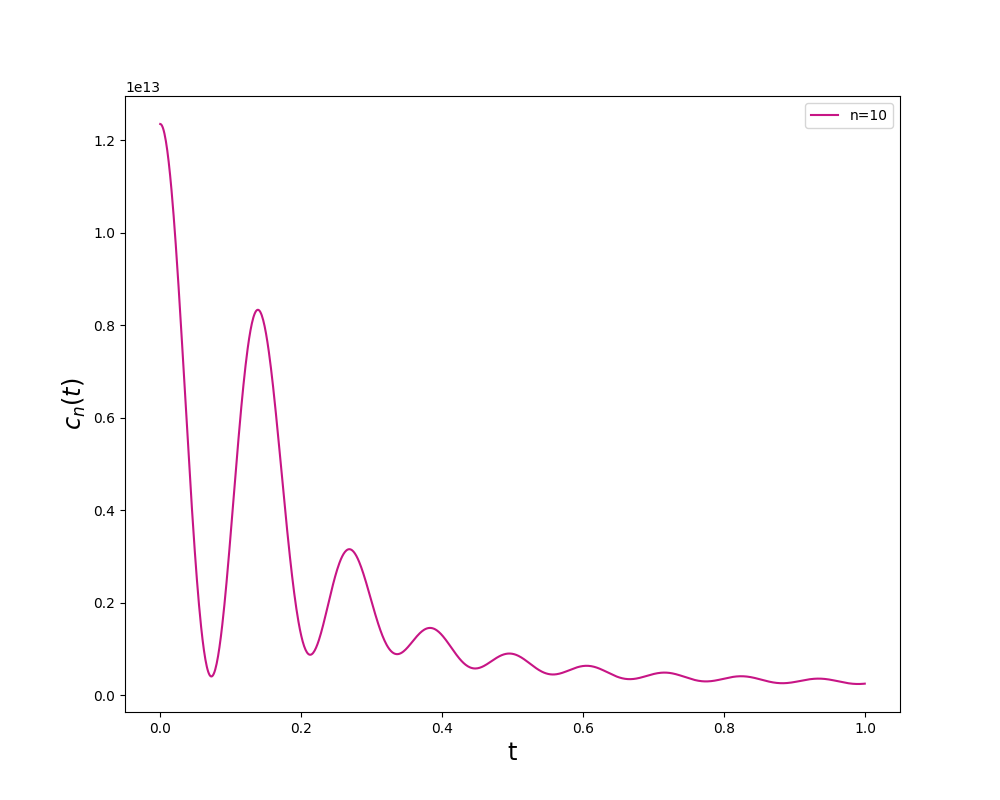
\includegraphics[width=0.6\textwidth]{pic1}
        \end{adjustbox}

        \begin{adjustbox}{center,caption={},label={microcanocnial OTOC},nofloat=figure,}
            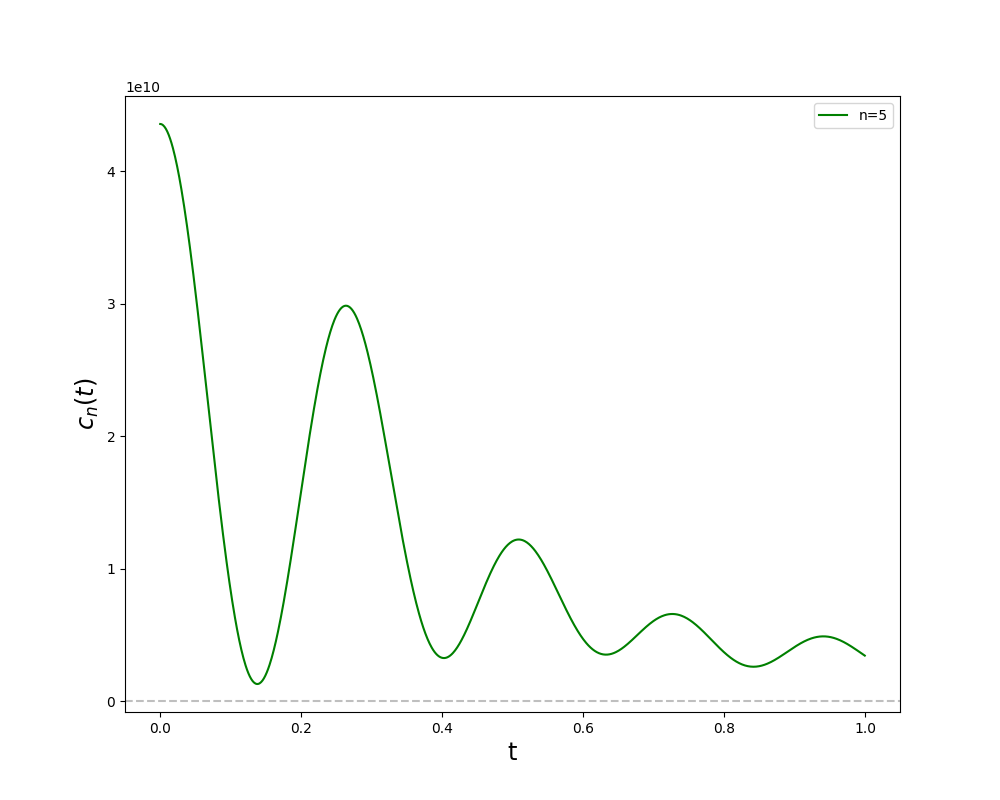
\includegraphics[width=0.6\textwidth]{pic2}
        \end{adjustbox}

        Here microcanonical OTOC and thermal OTOC are same with different temperatures.

        \lstinputlisting[language=Python, caption=Python example]{test14.py}
        
        \section{Conclusions}

        In this paper, we discussed what is Riemann hypothesis is, and why it is important to the field to Quantum mechanics. The imaginary part of Hamiltonian proposed by 
        Berry-keating Hamiltonian $H_{0} = \frac{1}{2}(xp+px)$ shows the self-adjoint and quanutm chaos. We look at Sierra regularization of Berry-Keating Hamiltonian, and 
        their intervals $l_{x}=1, \Lambda=1$ and evaluated the spectrum $E_{n} = \frac{2\pi \hbar}{ln \ N}(n+\frac{\theta}{2\pi})$ of $\psi_{E}(x) = \frac{C}{x^{\frac{1}{2}-iE\hbar}}$
        eigenfunction. Then we look at the quantization of inverse Hamiltonian $H_{0}^{-1} = x^{-1/2}p^{-1}x^{1/2} $ and obtained the spectrum $E_{n} = \frac{2\pi \hbar}{ln \ N}(n+\frac{1}{2})$
        which is reckon to be $E_{n} = \frac{2\pi \hbar}{ln \ N}(n+\frac{\theta}{2\pi})$ with $\theta = \pi$

        We discussed OTOC in quantum mehcanics and it thermal and microcanonical relation between them. We input the spccetrum and position operator of inverse Hamiltonaian 
        and calculate its quantum chaos analytically. We see that microcanonical OTOC settles at value greater than zero while the thermal OTOC displays the same behaviour
        of microcanonical OTOC.
    \bibliographystyle{plain}
    \bibliography{ref.bib}
\end{document}